\section{TaskBatch}

\subsection{Código}

\begin{lstlisting}[language=C++, breaklines=true]
void TaskBatch(int pid, vector<int> params) {

	srand(1); // set seed

	int total_cpu = params[0];
	int cant_bloqueos = params[1];

	bool config[total_cpu];
	fill_n(config, total_cpu, false);
	for (int i = 0; i < cant_bloqueos; i++) config[i] = true;
	random_shuffle(&config[0], &config[total_cpu-1]);

	for (int i = 0; i < total_cpu; ++i) {
		if (config[i] == true) { // block
			uso_IO(pid, 1);
		} else {
			uso_CPU(pid, 1);
		}
	}
}
\end{lstlisting}

El código que simula la tarea \texttt{TaskBatch} recibe dos parametros, estos son la cantidad de total de ciclos de reloj que lleva ejecutar la tarea y la cantidad de llamadas bloqueantes que ocurriran durante la ejecucion de la misma. A partir de la cantidad total de ciclos de CPU, se arma un vector en donde van a estar colocados los momentos donde ocurra una llamada bloqueante, estos se colocan de manera pseudoaleatoria con la funcion \texttt{random\_shuffle}. Una vez que termine este proceso, procedemos a simular la ejecucion de los ciclos de CPU utilizando el vector, si este indica que se debe producir una llamada bloqueante hace una llamada a \texttt{uso\_IO}, en el caso contrario se ejecuta un ciclo de CPU.

\subsubsection{Diagrama GANTT}

El siguiente diagrama fue generado con los siguientes parametros:

\begin{enumerate}
	\item lote\_tsk: 3.tsk
	\item num\_cores: 1
	\item switch\_cost: 4
	\item sched\_class: SchedFCFS
\end{enumerate}

\begin{figure}[h]
    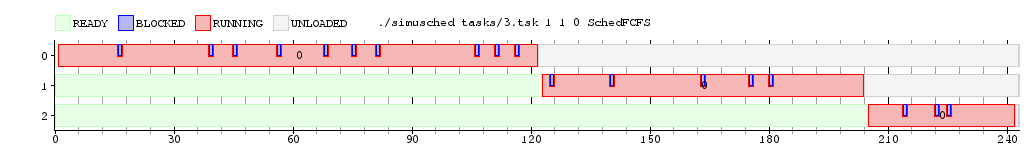
\includegraphics[width=\linewidth]{images/3.png}
    \label{fig:Task Consola}
    \caption{Task Batch}
\end{figure}

En la figura 4 se muestra el diagrama de Gantt de la ejecución de tareas del lote 3 bajo el scheduler FCFS, y con un \textit{switch cost} igual a 4. El lote en cuestión sólo cuenta con tareas de tipo \texttt{TaskBatch}, que utilizan una cantidad exacta de \textit{total\_cpu} ciclos de CPU y \textit{cant\_bloqueos} bloqueos, de un (1) ciclo cada una. En particular fueron ejecutadas con los siguientes parametros:

\begin{itemize}
	\item Tarea 0: 100 ciclos de CPU, 10 llamadas bloqueantes
	\item Tarea 1: 70 ciclos de CPU, 5 llamadas bloqueantes
	\item Tarea 2: 30 ciclos de CPU, 3 llamadas bloqueantes
\end{itemize}

Debido a que se trata del FCFS las tres tareas son ejecutadas secuencialmente, de modo que ejecuta la tarea siguiente únicamente tras finalizar la que actualmente figure en estado \textit{runing}. Para ello la proxima tarea a ejecutarse no sólo deberá aguardar los exactamente \textit{total\_cpu} ciclos de uso de CPU (que suelen carácterizar éste tipo de tareas) mas algún costo de cambio de contexto, sino que además tendrá que esperar otros \textit{cant\_bloqueos} ciclos, debido a las llamadas bloqueantes. A diferencia del ejercicio anterior, en este caso las llamadas bloqueantes demoran una cantidad preestablecida de ciclos, por lo que podemos conocer con total precisión la latencia de cada tarea.
\\
\\
\textsf{Latencias:}
\begin{itemize}
	\item Tarea 0: 4 ciclos
	\item Tarea 1: 118 ciclos
	\item Tarea 2: 197 ciclos 
\end{itemize}
